% Source printed p. 161, 400 DPI. Preserve the original uncaptioned illustration.
\begin{tikzpicture}
\node[anchor=south west,inner sep=0] (art) at (0,0)
{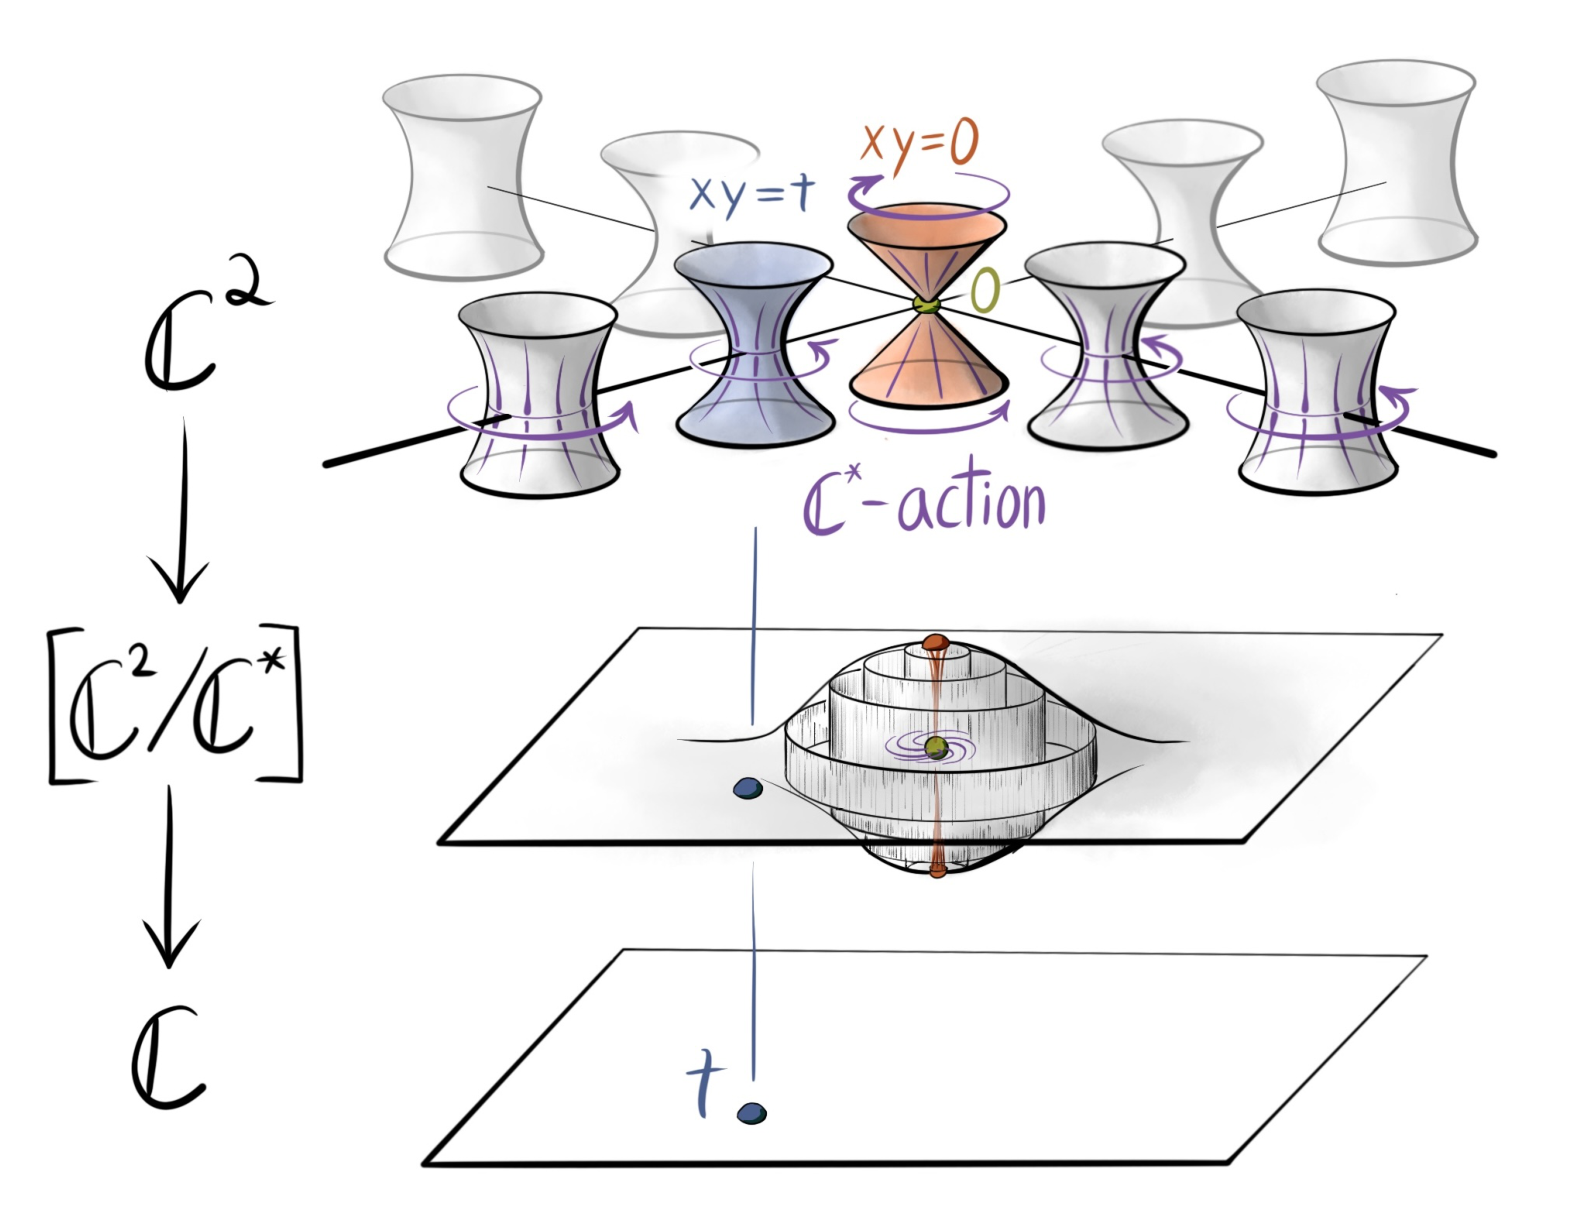
\includegraphics[width=.64\textwidth]{figures/fig-4.9.29.png}};
\begin{scope}[x={(art.south east)},y={(art.north west)}]
\fill[white] (0,0) rectangle (.205,1);
\node at (.105,.44) {\begin{tikzcd}[row sep=4.8em]
\mathbb C^2\arrow[d]\\
{[\mathbb C^2/\mathbb C^*]}\arrow[d]\\
\mathbb C
\end{tikzcd}};
\fill[white] (.50,.557) rectangle (.68,.628);
\node[text=violet,font=\small] at (.59,.593) {$\mathbb C^*$-作用};
\end{scope}
\end{tikzpicture}
